\documentclass[10pt]{beamer}

\usepackage{graphicx}
\usepackage{hyperref}
\usepackage{mathtools}
\DeclarePairedDelimiter{\ceil}{\lceil}{\rceil}
\usepackage{xcolor}
\graphicspath{{./images/}}

\usetheme{metropolis}
\setbeamertemplate{frame numbering}[fraction]
\useoutertheme{metropolis}
\useinnertheme{metropolis}
\usefonttheme{metropolis}
\usecolortheme{spruce}

\title{Undergraduate Seminar Presentation}
\subtitle{Expander Graphs}
\author{Karen Arzumanyan}
\date{November 1, 2021}

\begin{document}
\metroset{block=fill}

\begin{frame}
\maketitle
\end{frame}

\begin{frame}[t]{Graphs}
    \vspace{2em}
    What is a graph?
    \vspace{3em}
    \pause{}
    \begin{block}{Graph}
        A graph G is determined by a set of vertices V and a set of edges E that connect the elements of V together. \\
        An edge $e \in E$ that connects the vertices $v_1,v_2 \in V$ is denoted by $(v_1, v_2)$.
    \end{block}
    
\end{frame}

\begin{frame}[t]{Graphs}
    \textbf{Example:}\\
    \begin{figure}
        \centering
        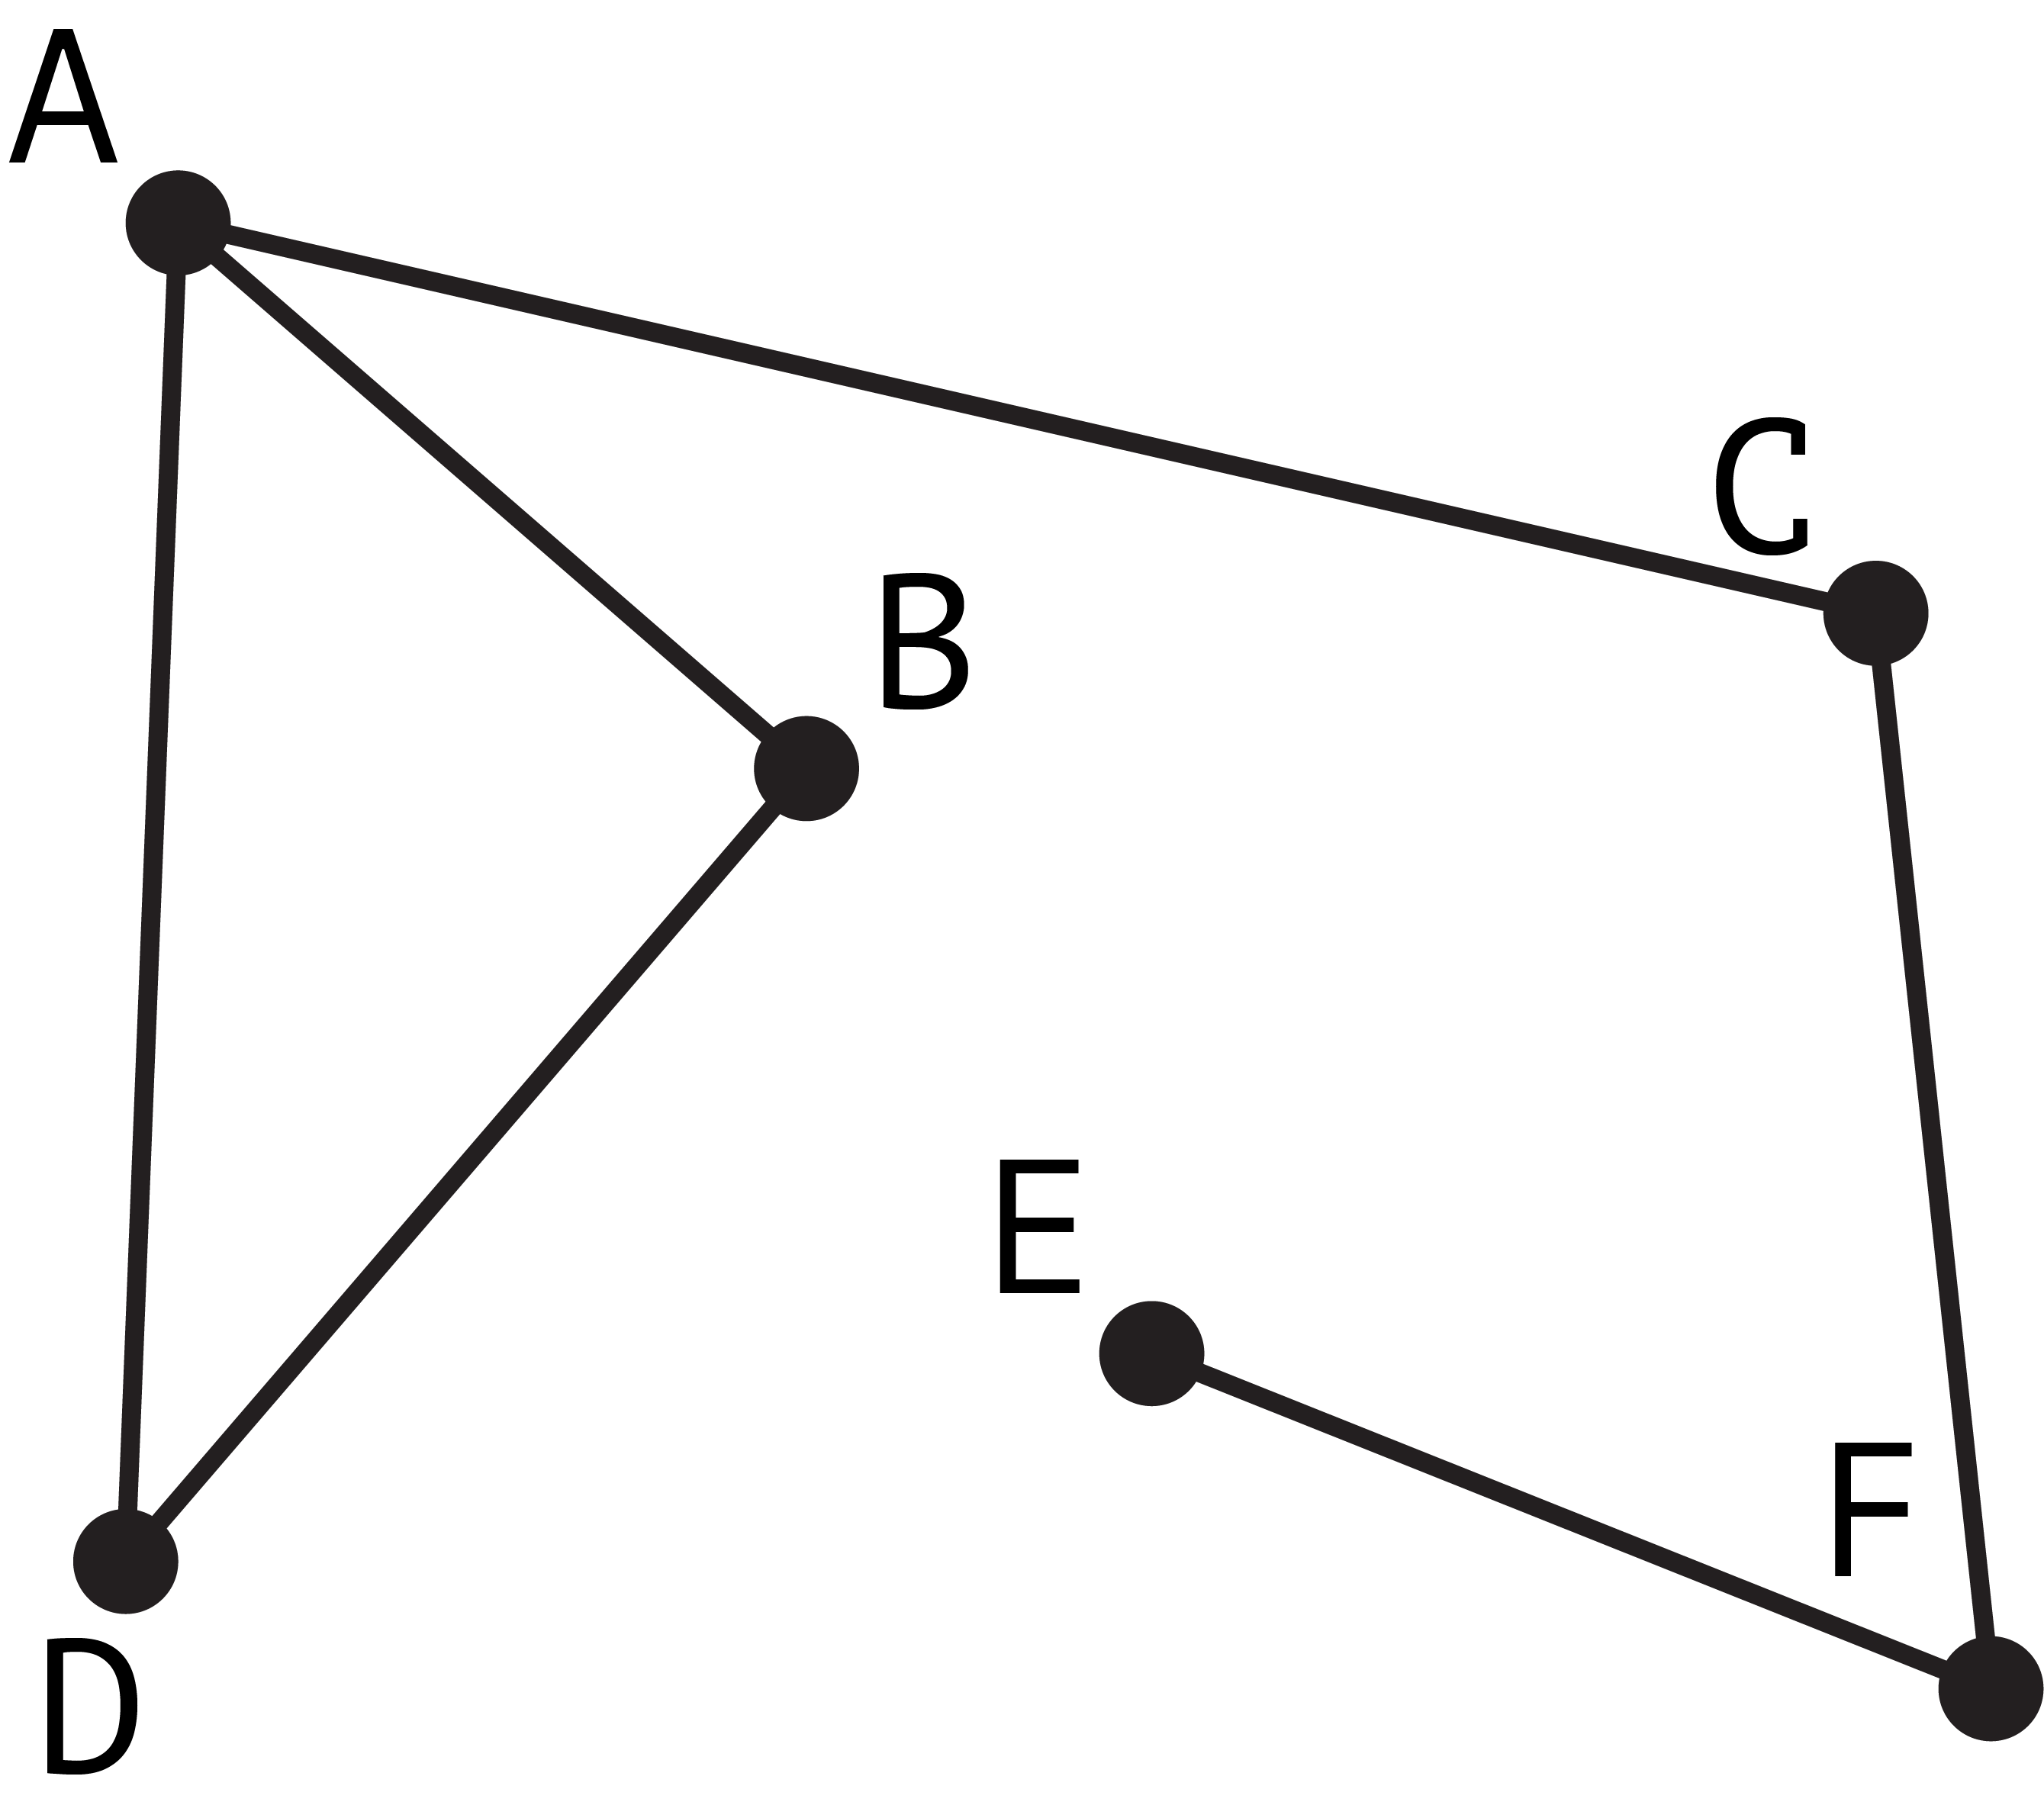
\includegraphics[width=120pt]{Graph}
        \caption{A graph consisting of 6 vertices and 6 edges.}
    \end{figure}
    \pause{}
    $V = \{A, B, C, D, E, F\}$\\
    \pause{}
    $E = \{(A,B), (A,C), (A,D), (C, F), (D, B), (E, F)\}$
\end{frame}

\begin{frame}[t]{Expander Graphs}
    \vspace{7em}
    \begin{block}{Informal Definition: Expander Graph}
        \vspace{0.5em}
        A graph G = (V, E) is called an \textit{expander graph} if every $S \subset V$ has its vertices connected to many verticies in $\bar{S} \subset V$.\newline Where $\bar{S} = V - S$.
        \vspace{0.5em}
    \end{block}
\end{frame}

\begin{frame}[t]{d-Regular Graphs}
    \begin{block}{Definition: d-Regular Graphs}
        \vspace{0.5em}
        A graph G is called \textit{d-Regular} if and only if every $v \in V$ is connected to $d$ other vertices in $V$.
        \vspace{0.5em}
    \end{block}
    \vspace{2pt}
    \pause{}
    \textbf{Example:}
    \begin{figure}
        \centering
        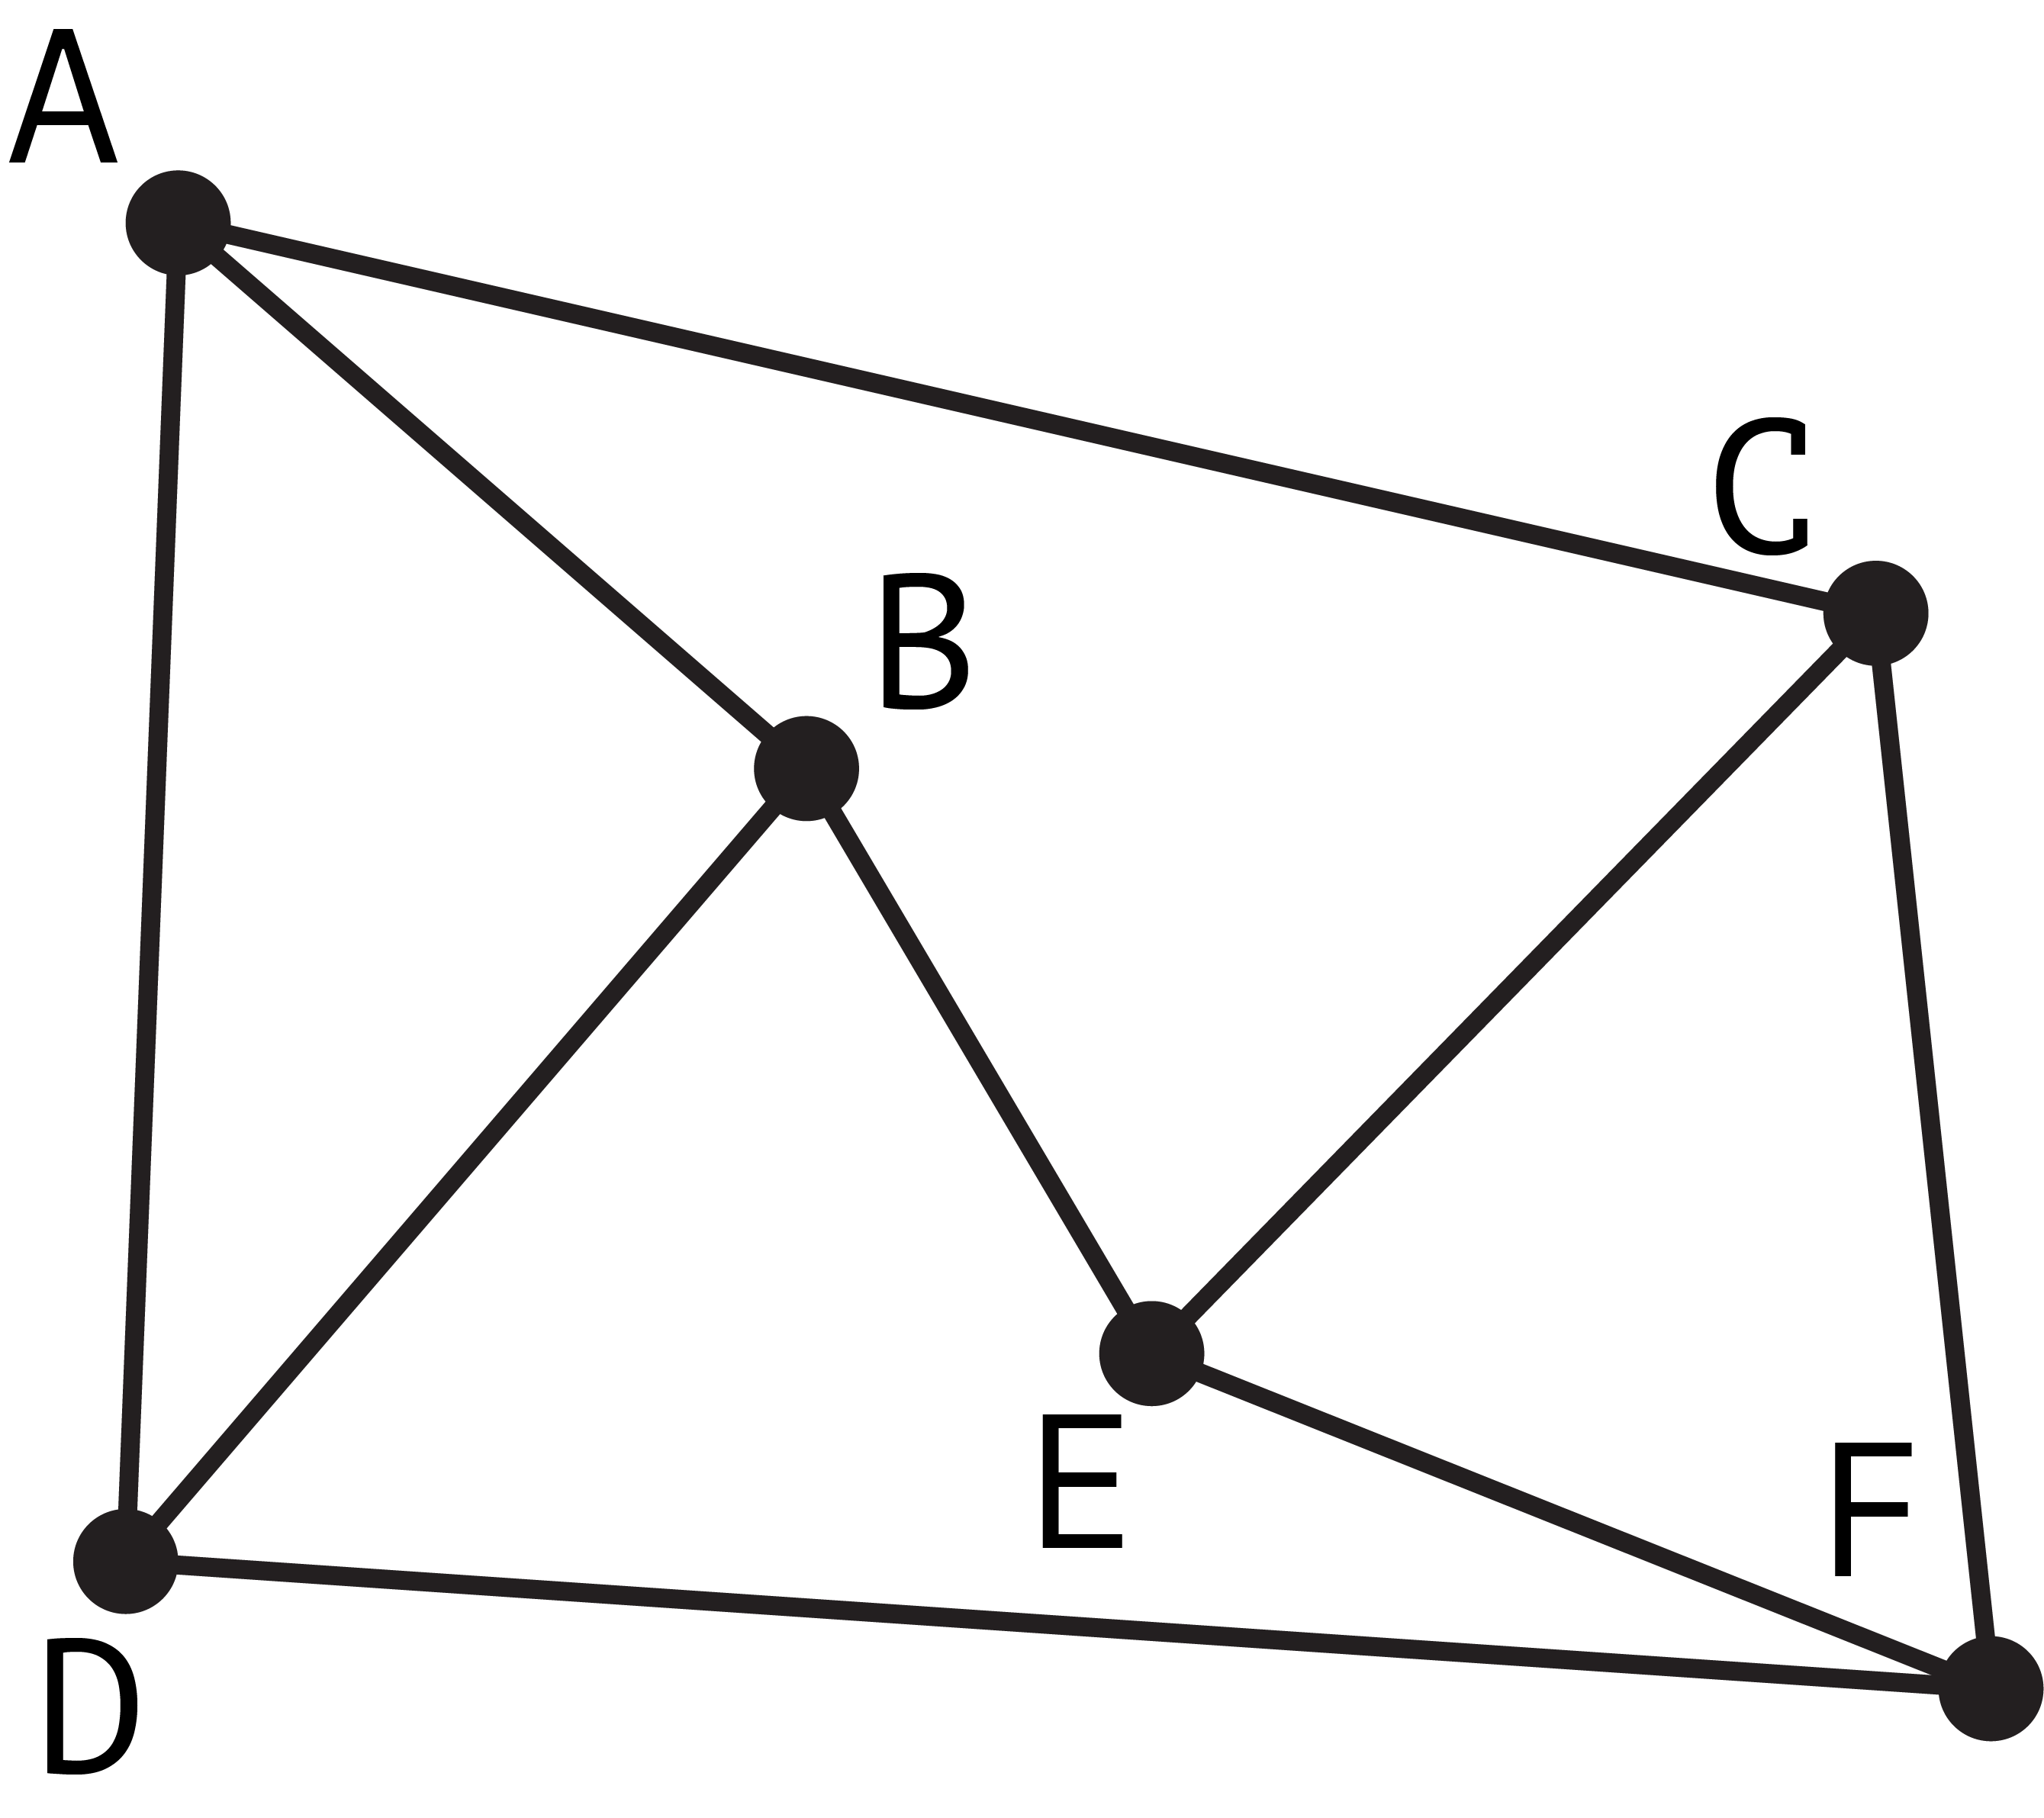
\includegraphics[width=120pt]{dGraph}
        \caption{A d-Regular graph where d is 3.}
    \end{figure}
\end{frame}

\begin{frame}[t]{Edge Boundary and Edge Expansion}
    \begin{block}{Edge Boundary}
        For a subset $S$ of $V$ we define the \textit{edge boundary} of $S \subset V$ to be the set of edges connecting S to its complement, $\bar{S}$. We denote the \textit{edge boundary} of $S$ as $\partial S$.
        \[\partial S = \{\ (v, w)\ |\ v \in S \text{ and } w \not \in S\ \}\]
    \end{block}
    \pause{}
    \begin{block}{Edge Expansion Parameter (also known as the Cheeger Constant)}
        We define a function \[h(G) \equiv \min\limits_{S:|S|\leq \frac{n}{2}} \frac{|\partial S|}{|S|}\text{.}\]
        $h(G)$ is the smallest possible ratio between the size of the \textit{edge boundary} of $S \subset V$ and the size of $S$ with $|S| \leq \frac{n}{2}$.
    \end{block}
\end{frame}

\begin{frame}[t]{Edge Boundary and Edge Expansion}
    \textbf{Example 1:} Suppose $G$ is a graph consisting of $n$ vertices, such that each vertex is connected to every other vertex (also known as a complete graph). Then for any two vertices $v \in S \text{ and } w \in \bar{S}$ there exists an edge $e \in E$ such that $e=(v,w)$.\\
    \vspace{5pt}
    \pause{}
    Thus, we can compute that $|\partial S|=|S| \times |\bar{S}|=|S|(n-|S|)$.\pause\\
    \vspace{5pt}
    Substituting this to the formula of $h(G)$ we get\\
    \[h(G)=\min\limits_{S:|S|\leq \frac{n}{2}} n - |S| = \ceil[\Big]{\frac{n}{2}}\text{.}\]
\end{frame}

\begin{frame}[t]{Edge Boundary and Edge Expansion}
    \textbf{Example 2:} Suppose that G is an $n\times n$ lattice in 2 dimensions, with periodic boundary conditions (so that G is 4-regular). Then if we consider a large connected subset $S \subset V$, it ought to be plausible that the \textit{edge boundary} set $\partial S$ will contain roughly one edge for each vertex on the perimeter of the region S. We expect there to be roughly $\sqrt{|S|}$ such vertices. 
    \pause{} Thus\\
    \[\frac{|\partial S|}{|S|} \approx \frac{\sqrt{|S|}}{|S|} = \frac{1}{\sqrt{|S|}}\]
    \pause{}
    We know that $S$ may contain up to $O(n^{2})$ elements.
    \pause{}
    Therefore
    \[h(G) = O\Big(\frac{1}{n}\Big)\]\\
    \pause{}
    \textbf{NOTE:} In this example, $\lim\limits_{n \rightarrow \infty} h(G) = 0$
\end{frame}

\begin{frame}{Edge Boundary and Edge Expansion}
    \begin{figure}
        \centering
        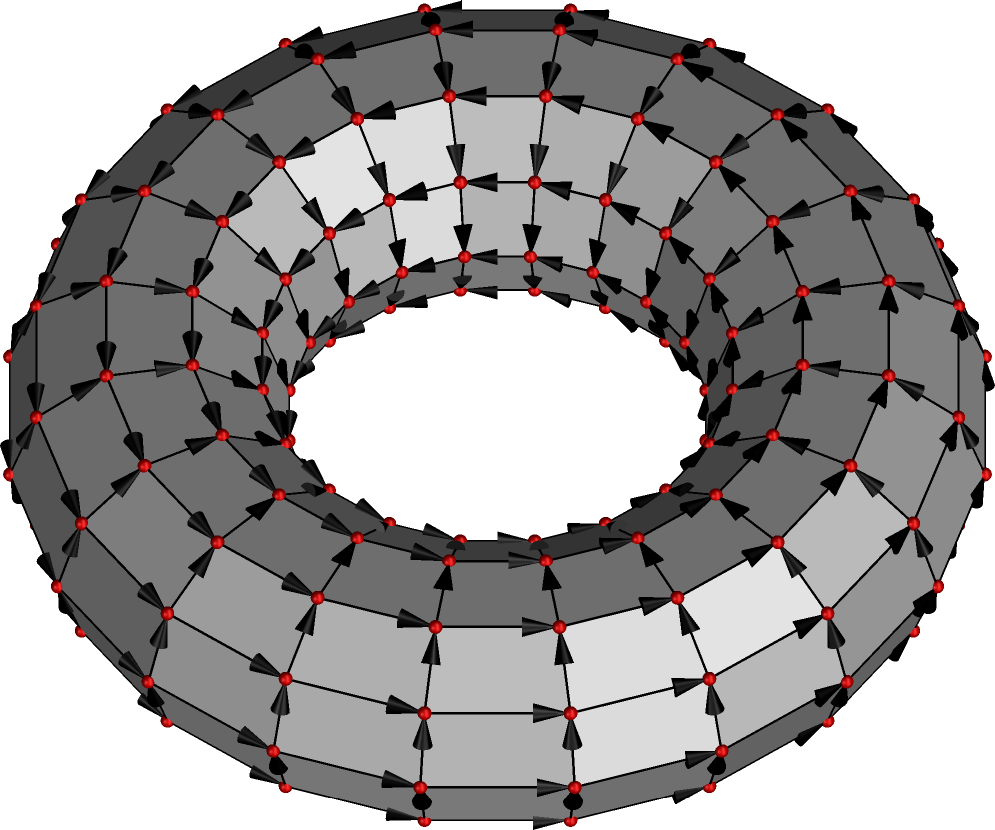
\includegraphics[width=200pt]{iu}
        \caption{A lattice graph with a periodic boundary condition in 3D.}
        %https://tex.stackexchange.com/a/148532 source
    \end{figure}
\end{frame}

\begin{frame}[t]{Edge Boundary and Edge Expansion}
    \textbf{Example 3:} Consider a d-regular graph G. Let all vertices in $V$ be connected to $d$ other \textit{random} vertices. Let $S \subset V$ consisting of at most $\frac{n}{2}$ vertices. 
    \pause{}
    Then, a vertex in $S$ will be connected to roughly $d \times \frac{|\bar{S}|}{n}$ vertices in $\bar{S}$. We expect $|\partial S| \approx d \frac{|S|\times|\bar{S}|}{n}$, \pause{}
    thus \[\frac{|\partial S|}{|S|} \approx \frac{1}{|S|} \times d\frac{|S|\times|\bar{S}|}{n} = d\frac{|\bar{S}|}{n}\]
    \pause{}
    But since $|\bar{S}|$ has its minimum at approximately $\frac{n}{2}$, 
    \pause{}
    we plug that value into our $h(G)$ approximation and get \[h(G) \approx d\frac{|\bar{S}|}{n} = d \frac{n}{2} \times \frac{1}{n}=\frac{d}{2}\]
    \pause{}
    \[h(G) \approx \frac{d}{2}\]
\end{frame}

\begin{frame}[t]{Expander Graphs}
    \vspace{5em}
    \begin{block}{Definition: Expander Graph}
        If we have a family $G_j = (V_j, E_j)$ of \textit{d}-regular graphs, indexed by \textit{j}, and such that $|V_j|=n_j$ for some increasing sequence $n_j$. Then we say that the family $\{G_j\}$ is a \textit{family of expander graphs} if the edge expansion parameter is bounded strictly away from 0, i.e, there is some (small) constant $c$ such that $h(G_j) \geq c > 0$ for all $G_j$ in the family.
    \end{block}
\end{frame}

\begin{frame}[t]{Expander Graphs}
    \textbf{Example:} Consider a family of graphs indexed by a prime number $p$. The set of vertices for the graph $G_p$ is just the set of points in $Z_p$, the field of integers modulo p. 
    \pause{}
    We construct a 3-regular graph by connecting each vertex $x \neq 0$ to $x-1$, $x+1$, and $x^{-1}$.
    \pause{}
    The vertex $x=0$ is connected to $p-1$, $0$, and $1$.
    \pause{}
    This is proven to be a family of expander graphs by Lubotsky, Philips, and Sarnak in 1988.
\end{frame}

\begin{frame}{Adjacency Matrix}
    \vspace{3em}
    \begin{block}{Adjacency Matrix}
        The rows and columns of the Adjacency Matrix are labelled by the vertices of V.\\
        More precisely, $A(G)$ is the adjacency matrix of the graph $G=(V, E)$. Then for vertices $v,w \in V$ the entry $A(G)_{vw} = 1$ if $(v,w)$ is an edge, i.e $(v,w) \in E$; likewise, $A(G)_{vw} = 0$ if $(v,w)$ is not an edge, i.e. $(v,w) \not \in E$.
    \end{block}
    \end{frame}

\begin{frame}[t]{Eigenvalues}
    \vspace{2em}
    Assuming that the graph G is a finite graph with n vertices, then A(G) is an $n \times n$ symmetric  matrix.
    \pause{}
    Therefore, $A(G)$ has n real eigenvalues, counting multiplicities.
    \pause{}
    $$\lambda_1 \geq \lambda_2 \geq \ldots \geq \lambda_n$$
    \pause{}
    Furthermore, if $G$ is d-regular, then the largest eigenvalue of $A(G)$ is $d$.
    \pause{}
    \vspace{3em}
    \begin{block}{Definition: Spectrum of a  Graph}
        The spectrum of the graph G is the set of all \textit{eigenvalues} of $A(G)$.
    \end{block}
\end{frame}

\begin{frame}{Connectivity of a d-regular Graph}
    \begin{block}{Proposition} A d-regular graph G is connected if and only if $\lambda_1(G) > \lambda_2(G)$.
    \end{block}
    \pause{}
    \begin{block}{Proof}
        We prove by contrapositive, namely, that a d-regular \textit{disconnected} graph has $\lambda_1(G) = \lambda_2(G)$.
        \pause{}
        We break up the graph $G$ into disconnected components $G_1$ and $G_2$. We can observe that $A(G) = A(G_1) \bigoplus A(G_2)$.
        \pause{}
        Since both $G_1$ and $G_2$ are d-regular, their largest eigenvalues are $d$, which means that $d$ appears (at least) twice in spectrum of $A(G)$.
    \end{block}
\end{frame}

\begin{frame}{Gap and Expansion}
    \begin{block}{Definition: Gap of the graph  G}
        We define the \textit{gap for the graph G} to be the difference $\Delta(G) 
        \equiv \lambda_1(G) - \lambda_2(G)$ between the largest and the second-largest eigenvalues.
    \end{block}
    \pause{}
    \begin{block}{Theorem}
        The expansion parameter $h(G)$ for a d-regular graph G is related to the gap $\Delta(G)$ by:
        $$\frac{\Delta(G)}{2} \leq h(G) \leq \sqrt{2d\Delta(G)}$$
    \end{block}
    \pause{}
    \begin{block}{Remark}
        If the gap for a family of d-regular graphs is bounded below by a positive constant, then the expansion parameter must also be bounded below by a positive constant, thus showing that the family is expander.
    \end{block}
\end{frame}

\begin{frame}[t]{Gap and Expansion}
    \begin{block}{Proof Sketch of the Theorem}
        We already know that $\lambda_1(G) = d$ with eigenvector $\vec{1} = (1,1,\ldots,1)$.
        \pause{}
        So we will now try to understand the behavior of $\lambda_2(G)$.
        \pause{}
        A way to gain control over $\lambda_2(G)$ is to observe that it is just the maximum of the expression
        $$v^TA(G)v/v^Tv$$
        where we maximize over all vectors $v$ orthogonal to the eigenvector $\vec{1}$.
    \end{block}
\end{frame}

\begin{frame}{Gap and Expnansion}
    \begin{block}{Proof Sketch of the Theorem Continued}
        Using the fact that if $v$ is orthogonal to $\vec{1}$ is only possible if the sum of $v$'s entries is equal to 0.
        \pause{}
        Thus we have,
        $$\lambda_2(G) = \max\limits_{v:tr(v)=0} \frac{v^TA(G)v}{v^Tv}$$
        where $tr(v)$ is the sum of entries of the vector v.\\
        \pause{}
        We can provide a lower bound on $\lambda_2(G)$ by simply guessing a good choice of v satisfying $tr(v)=0$, in addition to using the fact
        $$\lambda_2(G) \geq \frac{v^TA(G)v}{v^Tv}.$$
    \end{block}
\end{frame}

\begin{frame}{Gap and Expnansion}
    \begin{block}{Proof Sketch of the Theorem Continued}
        To make a good guess, we need a convenient way to look at $v^TA(G)v$, where $tr(v)=0$.
        \pause{}
        Let's think of $v$ as the difference of two disjoint probability distributions, $p$ and $q$, which means that $v=p-q$, where $p$ and $q$ are non-negative vectors each summing to 1 and having disjoint support.
        \pause{}
        Now let's define a vector $\vec{1}_S$ to be the vector whose entries are 1 on S, and 0 elsewhere.
    \end{block}
\end{frame}

\begin{frame}{Gap and Expnansion}
    \begin{block}{Proof Sketch of the Theorem Continued}
        Now we can observe that 
        \[\vec{1}_S^TA(G)\vec{1}_T = |E(S,T)|\text{,}\]
        where $E(S,T)$ is the number of edges between the vertex sets S and T.
        \pause{}
        This means that we should choose $p$ and $q$ in terms of vectors like $\vec{1}_S$, since it will enable us to relate expressions such as $v^TA(G)v$ to the sizes of various edge sets, which are how we will relate to the expansion parameter.
        \pause{}
        Suppose we chose \[v=\frac{\vec{1}_S}{|S|}-\frac{\vec{1}_{\bar{S}}}{|\bar{S}|}\]
        \pause{}
        This satisfies the condition tr(v)=0, and leaves us with
        \[v^Tv=\frac{1}{|S|}+\frac{1}{|\bar{S}|}\]
    \end{block}
\end{frame}

\begin{frame}{Gap and Expnansion}
    \begin{block}{Proof Sketch of the Theorem Continued}
        This in fact shows us that
        \[v^TA(G)v = \frac{1}{{|S|}^2}E(S,S) + \frac{1}{{|\bar{S}|}^2}E(\bar{S},\bar{S})-\frac{2}{|S||\bar{S}|}E(S,\bar{S})\]
        \pause{}
        By the definition of an expander graph, we have control over $E(S,\bar{S})$, so we can rewrite $E(S,S)$ and $E(\bar{S},\bar{S})$ in terms of $E(S,\bar{S})$, using the \textit{d}-regularity of the graph.
        \pause{}
        We get, 
        \[E(S,S)+E(S,\bar{S})=d|S| \text{ and } E(\bar{S},\bar{S})+E(S,\bar{S})=d|\bar{S}|\]
    \end{block}
\end{frame}

\begin{frame}{Gap and Expnansion}
    \begin{block}{Proof Sketch of the Theorem Continued}
        Now if we substitute our findings into $v^TA(G)v$, we get
        \[v^TA(G)v=d\Big(\frac{1}{|S|}+\frac{1}{|\bar{S}|}\Big)-\Big(\frac{1}{|S|}+\frac{1}{|\bar{S}|}\Big)^2E\Big(S,\bar{S}\Big)\]
        \pause{}
        And then comparing with the earlier expression for the denominator $v^Tv$, we obtain
        \[\lambda_2(G) \geq d - \Big(\frac{1}{|S|}+\frac{1}{|\bar{S}|}\Big)E(S,\bar{S})\]
        \pause{}
        Now we choose S such that $E(S,\bar{S}) = h(G)|S|$ and $|S| \leq \frac{n}{2}$.
        \pause{}
        After substituting and performing a little bit of algebra, we get
        \[\lambda_2(G) \geq d-2h(G)\text{,}\]
        \pause{}
        and thus
        \[\frac{\Delta(G)}{2} \leq h(G)\text{.}\]
    \end{block}
\end{frame}

\begin{frame}{Gap and Expnansion}
    We only proved the lower bound.\\
    \pause{}
    The proof of the upper bound is too complicated and time consuming, so it can be found in the notes of Linial and Wigderson.
\end{frame}

\begin{frame}{What comes next?}
    \begin{block}{Random Walks on Expanders}
        You choose some vertex in an expander graph G, and then repeadetly move to one of its $d$ neighbors, while choosing uniformly at random, as well as, independent of previous choices.
    \end{block}
    For more details see \cite{N}\\
    \vspace{2em}
    Most applications of expanders utilize the random walks.
\end{frame}

\begin{frame}{Applications of Expander Graphs}
    \begin{itemize}
        \item \textbf{\textit{Reduce the need for randomness:}} That is, expanders can be used to reduce the number of random bits needed to make a probabilistic algorithm work with some desired probability.
        \item \textbf{\textit{Find good error-correcting codes:}} Expanders can be used to construct error correcting codes for protecting information against noise. Expanders can be used to find error correcting codes which are efficiently encodable and decodable. Finding codes with such properties was one of the milestone in information theory.
    \end{itemize}
\end{frame}

\begin{frame}{Work Cited}
    \begin{thebibliography}{3}
        \bibitem{N} Nielsen, M. A., \href{https://michaelnielsen.org/people/nielsen/blog/archive/notes/expander\_graphs.pdf}{Introduction to expander graphs}.
        \bibitem{G} G. Davidoff, P. Sarnak, and A. Valette. \textit{Elementary number theory, group theory, and Ramanujan graphs}, volume 55 of London Mathematical Society Student Texts. Cambridge University Press, Cambridge, 2003.
    \end{thebibliography} 
\end{frame}
\end{document}

